\documentclass[a5paper]{book}
\usepackage[nottoc,numbib]{tocbibind}
\usepackage[english]{babel}
\usepackage[pdftex]{graphics} %enable pdfgraphics support necessary for pdflatex
\usepackage{graphicx}
\usepackage{tikz}
\usepackage[small,bf]{caption}
\usepackage{footmisc}
\usepackage{sidecap}
\usepackage{fancyvrb}
\usepackage{color}
\usepackage{rotating}
\makeatletter
\setlength{\@fptop}{0pt}
\setlength{\@fpsep}{5pt}
\makeatother
\renewcommand{\dotfill}{\leaders\hbox to 5pt{\hss.\hss}\hfill}
\usepackage[hmargin=1.2cm,vmargin=1.5cm]{geometry} %set custom margins
\usepackage{fancyhdr} %enable hyperlinking, highlight page numbers
\usepackage{amsmath}
\usepackage{amssymb}
\numberwithin{equation}{subsection}
\usepackage{amsfonts}
\usepackage{mathrsfs}
\usepackage{tabularx}
\usepackage{lastpage}
\usepackage{subfigure}
\usepackage{multicol}
\usepackage{lipsum}
\usepackage{xspace}
\usepackage{latexsym} 
\usepackage{verbatim}
\usepackage{listings}
\usepackage{color}
\usepackage[usenames,dvipsnames]{xcolor}
\definecolor{listinggray}{gray}{0.9}
\definecolor{lbcolor}{rgb}{0.9,0.9,0.9}
\usepackage{listings}
\usepackage{color}

\definecolor{mygreen}{rgb}{0,0.6,0}
\definecolor{mygray}{rgb}{0.5,0.5,0.5}
\definecolor{mymauve}{rgb}{0.58,0,0.82}

\lstset{ %
   backgroundcolor=\color{white},   % choose the background color; you must add \usepackage{color} or \usepackage{xcolor}
   basicstyle=\footnotesize,        % the size of the fonts that are used for the code
   breakatwhitespace=false,         % sets if automatic breaks should only happen at whitespace
   breaklines=true,                 % sets automatic line breaking
%   captionpos=b,                    % sets the caption-position to bottom
   commentstyle=\color{mygreen},    % comment style
   deletekeywords={...},            % if you want to delete keywords from the given language
   escapeinside={\%*}{*)},          % if you want to add LaTeX within your code
   extendedchars=true,              % lets you use non-ASCII characters; for 8-bits encodings only, does not work with UTF-8
   frame=single,                    % adds a frame around the code
   keepspaces=true,                 % keeps spaces in text, useful for keeping indentation of code (possibly needs columns=flexible)
   keywordstyle=\color{blue},       % keyword style
   language=Octave,                 % the language of the code
   morekeywords={*,...},            % if you want to add more keywords to the set
   numbers=left,                    % where to put the line-numbers; possible values are (none, left, right)
   numbersep=5pt,                   % how far the line-numbers are from the code
   numberstyle=\tiny\color{mygray}, % the style that is used for the line-numbers
   rulecolor=\color{black},         % if not set, the frame-color may be changed on line-breaks within not-black text (e.g. comments (green here))
   showspaces=false,                % show spaces everywhere adding particular underscores; it overrides 'showstringspaces'
   showstringspaces=false,          % underline spaces within strings only
   showtabs=false,                  % show tabs within strings adding particular underscores
   stepnumber=1,                    % the step between two line-numbers. If it's 1, each line will be numbered
   stringstyle=\color{mymauve},     % string literal style
   tabsize=2,                       % sets default tabsize to 2 spaces
%   title=\lstname                   % show the filename of files included with \lstinputlisting; also try caption instead of title
}
% tweak the the style a little bit
\lstdefinestyle{customc}{
%   belowcaptionskip=1\baselineskip,
   breaklines=true,
   frame=single,
   xleftmargin=\parindent,
   language=C++,
%   showstringspaces=false,
   basicstyle=\footnotesize\ttfamily,
   keywordstyle=\bfseries\color{green!40!black},
   commentstyle=\itshape\color{mygray},
   identifierstyle=\color{blue},
   stringstyle=\color{orange},
   framexleftmargin=5mm,
}

\lstset{escapechar=@,style=customc}
\usepackage[sort&compress,numbers]{natbib}

\pagestyle{fancy} %enable custom headeres
\fancyhead{}
\fancyfoot{} %clear predefined headers, then create your own:
\lhead{\footnotesize AliROOT Flow Package manual and documentation}
\rhead{\footnotesize The FLOW team}
\rfoot{\footnotesize Page \thepage\ of \pageref{LastPage}}
\lfoot{\footnotesize \rightmark}
\usepackage[bookmarks=true,
            bookmarksopen=true, 
            bookmarksnumbered=true, pdftex,
            hyperindex=true,linktocpage]{hyperref}
\hypersetup{
    bookmarks=true,         % show bookmarks bar?
    unicode=false,          % non-Latin characters in Acrobat’s bookmarks
    pdftoolbar=true,        % show Acrobat’s toolbar?
    pdfmenubar=true,        % show Acrobat’s menu?
    pdffitwindow=false,     % window fit to page when opened
    pdfstartview={FitH},    % fits the width of the page to the window
    pdftitle={AliROOT Flow Package manual and documentation},    % title
    pdfauthor={Redmer Alexander Bertens},     % author
    pdfsubject={AliROOT Flow Package manual and documentation},   % subject of the document
    pdfcreator={Redmer Alexander Bertens},   % creator of the document
    pdfproducer={Redmer Alexander Bertens}, % producer of the document
    pdfkeywords={ALICE} {AliROOT} {ROOT} {manual} {flow} {package} {software}, % list of keywords
    pdfnewwindow=true,      % links in new window
    colorlinks=true,       % false: boxed links; true: colored links
    linkcolor=blue,          % color of internal links
    citecolor=green,        % color of links to bibliography
    filecolor=blue,      % color of file links
    urlcolor=blue           % color of external links
}
\usepackage{lineno}
\usepackage{makeidx}
\makeindex

\sloppy
\fancypagestyle{plain}
 {
 \fancyhead{}
 \fancyfoot{}
 } % clear header and footer of plain page because of ToC

 % tikxstyle for integration of tikz graphics
\tikzstyle{every node}=[font=\tiny]
\tikzstyle{decision} = [rectangle, draw, fill=yellow!20, 
    rounded corners, minimum height=1.5em, minimum width=2.5em, inner sep=3pt]
\tikzstyle{decision2} = [rectangle, draw, fill=red!20, 
    rounded corners, minimum height=1.5em, minimum width=2.5em, inner sep=3pt]
\tikzstyle{decision3} = [rectangle, draw, fill=green!20, 
    rounded corners, minimum height=1.5em, minimum width=2.5em, inner sep=3pt]
\tikzstyle{block} = [rectangle, draw, fill=blue!20, 
    rounded corners, minimum height=1.5em, minimum width=2.5em, inner sep=3pt]
\tikzstyle{line} = [draw, -latex']
\tikzstyle{cloud} = [draw, ellipse,fill=red!20, 
    minimum height=2em]
\tikzstyle{sdecision} = [rectangle, draw, fill=yellow!20, 
    rounded corners, minimum height=1.5em, minimum width=2.5em, inner sep=3pt]
\tikzstyle{sblock} = [rectangle, draw, fill=blue!20, 
    rounded corners, minimum height=1.5em, minimum width=2.5em, inner sep=3pt]
\tikzstyle{scloud} = [draw, ellipse,fill=red!20, 
    minimum height=2em]
\tikzstyle{ycloud} = [draw, ellipse,fill=yellow!20, 
    minimum height=2em]

\renewcommand{\thefootnote}{\fnsymbol{footnote}}
\frontmatter

\linenumbers
\begin{document}

\noindent
\begin{center}
	\vspace*{1.5cm}
	{\LARGE \bf The FLOW Analysis Package}\\
		
	\vspace{1.5cm}
	\begin{figure}[hbt]
		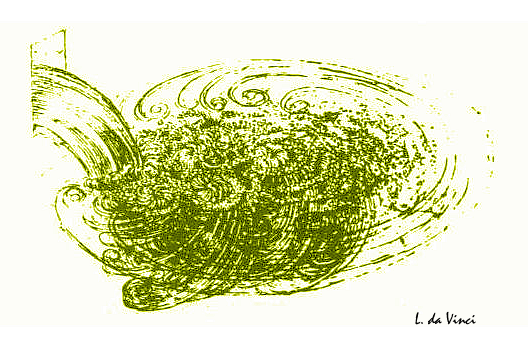
\includegraphics[width=1.\textwidth]{figs/daVinci.png}
	\end{figure}
		
	\vspace{1.5cm}
	\noindent
	{\large \bf a short writeup}\\
	\today\\
\end{center}
\vfill
\noindent
Various authors, edited by Redmer Alexander Bertens (\texttt{rbertens@cern.ch})

\clearpage
\thispagestyle{empty}
\pagenumbering{roman}
\tableofcontents
\renewcommand{\thefootnote}{\alph{footnote}}
\mainmatter
\chapter{Introduction}
The intro to everything.
%-----------------------------------------------------------------------
\chapter{A Quick Start}
\section{The flow package}
\label{quickstart}
The \texttt{ALICE flow package}\index{flow package}\index{ALICE flow package|see{flow package}}\footnote{The ALICE flow package is part of AliROOT\index{AliROOT}, the ALICE extension of the ROOT framework, which can be obtained from \href{http://git.cern.ch/pub/AliRoot}{http://git.cern.ch/pub/AliRoot}. The flow package itself is located in the folder \texttt{\$ALICE\_ROOT/PWG/FLOW/}, where \texttt{\$ALICE\_ROOT} refers to the source directory of AliROOT.} 
contains most known flow analysis methods.  In this chapter we give a few examples how to setup an
analysis for the most common cases. The chapters that follow provide more detailed information on the structure of the code 
and settings of the various flow methods. 
This write-up is however not a complete listing of the methods, for this the reader is referred to the header files.
 
\section{On the fly}
The macro \texttt{Documentation/examples/runFlowOnTheFlyExample.C}\index{On the fly}\index{runFlowOnTheFlyExample.C}\footnote{In aliroot, this macro can be found at \\ \texttt{\$ALICE\_ROOT/PWGCF/FLOW/Documentation/examples/runFlowOnTheFlyExample}} is a basic example of how the flow package works. 
In this section we explain the main pieces of that macro.
\begin{enumerate}
	\item To use the flow code the flow library needs to be loaded. In\index{libraries, AliROOT} \texttt{AliROOT}:
	\begin{lstlisting}
gSystem->Load("libPWGflowBase");\end{lstlisting}
	In \texttt{root} additional libraries need to be loaded\index{libraries, ROOT}: 
	\begin{lstlisting}
gSystem->Load("libGeom");
gSystem->Load("libVMC");
gSystem->Load("libXMLIO");
gSystem->Load("libPhysics");
gSystem->Load("libPWGflowBase");\end{lstlisting}
	\item We need to instantiate the flow analysis methods which we want to use. In this example we will
	instantiate two methods: the first which calculates the flow versus the reaction plane of the Monte Carlo, which is our reference value\index{reference value}\index{Monte Carlo Event Plane} (see section \ref{MC}), and second the so called Q-cumulant method (see section \ref{qvc}).
	\begin{lstlisting}
AliFlowAnalysisWithMCEventPlane *mcep = new AliFlowAnalysisWithMCEventPlane();
AliFlowAnalysisWithQCumulants *qc = new AliFlowAnalysisWithQCumulants();\end{lstlisting}
	\item Each of the methods needs to initialize\index{initialize methods} (e.g. to define the histograms): 
	\begin{lstlisting}
mcep->Init(); 
qc->Init();\end{lstlisting}
	\item To define the particles we are going to use as Reference Particles\index{reference particles} \index{RP|see{reference particles}} (RP's, particles 
	used for the {\bf Q} vector) and the Particles Of Interest\index{particles of interest} \index{POI|see{particles of interest}} (POI's, the particles of which 
	we calculate the differential flow) we have to define two track cut objects\index{track cut object, simple}:
	\begin{lstlisting}
AliFlowTrackSimpleCuts *cutsRP = new AliFlowTrackSimpleCuts();
AliFlowTrackSimpleCuts *cutsPOI = new AliFlowTrackSimpleCuts();
cutsPOI->SetPtMin(0.2);
cutsPOI->SetPtMax(2.0);	\end{lstlisting}
	\item Now we are ready to start the analysis. For a quick start we make an event on the fly, tag the reference particles and particles of interest  and pass it to the two flow methods. \\
	\begin{lstlisting}
for(Int_t i=0; i<nEvts; i++) { 
      // make an event with mult particles 
      AliFlowEventSimple* event = new AliFlowEventSimple(mult,AliFlowEventSimple::kGenerate);
      // modify the tracks adding the flow value v2
      event->AddV2(v2);
      // select the particles for the reference flow
      event->TagRP(cutsRP);
      // select the particles for differential flow
      event->TagPOI(cutsPOI);
      // do flow analysis with various methods:
      mcep->Make(event);
      qc->Make(event);
}\end{lstlisting}
	\item To fill the histograms which contain the final results we have to call Finish for each method:
	\begin{lstlisting}
mcep->Finish(); 
qc->Finish(); \end{lstlisting}
	\item This concludes the analysis and now we can write the results into a file. Two options for writing the input to a file are available: 
     \begin{itemize}
     \item Create a new output file and write the output to this file
     \begin{lstlisting}
TFile *outputFile = new TFile("mcep_ouput.root","RECREATE");
mcep->WriteHistograms();
TFile *outputFile = new TFile("qc_ouput.root","RECREATE");
qc->WriteHistograms();\end{lstlisting}
Please note that writing the 
\end{enumerate}

\section{What is in the output file?}
\index{output file}Now we have written the results into a file, but what is in there?

\section{Reading events from file}
The macro \texttt{Documentation/examples/runFlowReaderExample.C} \index{runFlowReaderExample.C}is an example how to setup a flow analysis if the events are already generated and
for example are stored in ntuples.
 
\section{A simple flow analysis in ALICE using Tasks}
The macro \texttt{Documentation/examples/runFlowTaskExample.C} \index{runFlowTaskExample.C}is an example how to setup a flow analysis using the full ALICE Analysis Framework.

%-----------------------------------------------------------------------

\chapter{The Flow Event}
\label{flowevent}
Here we describe the flowevent, flowtracks, general cuts and cuts for RPs POIs.
OntheFly, AfterBurner. Filling with ESD, AOD, Ntuples, etc.  
%-----------------------------------------------------------------------

\chapter{The Program}
\label{The Program}
\begin{center}
	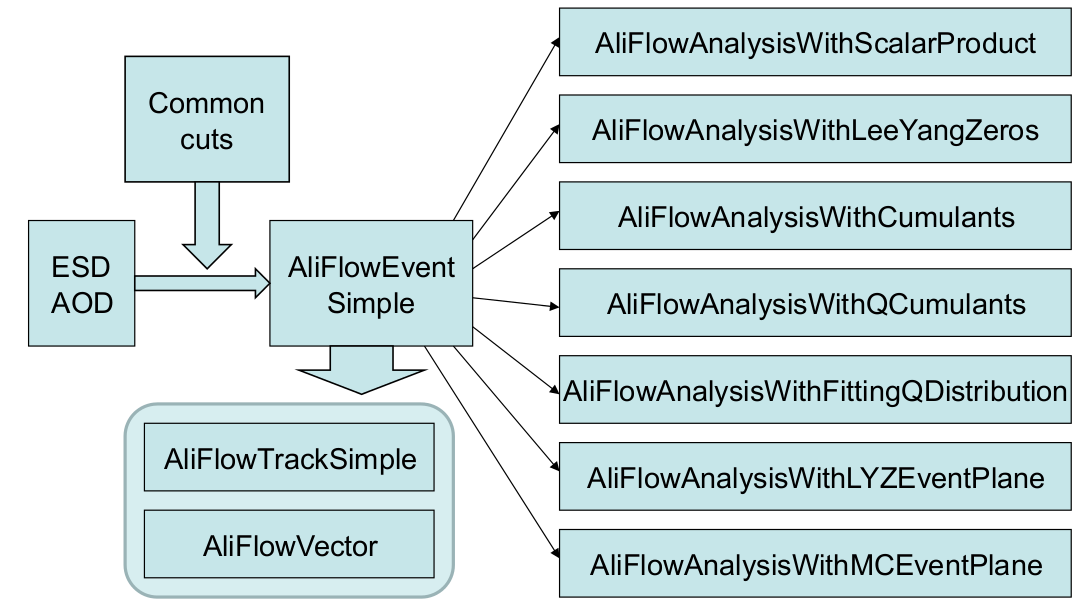
\includegraphics[width=1.\textwidth]{figs/flowChart.png}
\end{center}
Here we describe the program.
%-----------------------------------------------------------------------

\chapter{Methods}
\label{Methods}
The flow package aims at providing the user with most of the known flow analysis methods. Detailed theoretical overview of the methods can be found in the following papers, which are included in the folder \texttt{\$ALICE\_ROOT/PWGCF/FLOW/Documentation/otherdocs/}
\begin{itemize}
	\item The Monte-Carlo Truth
	\item Scalar Product Method \\ \hspace*{1cm} \texttt{EventPlaneMethod/FlowMethodsPV.pdf}
	\item Generating Function Cumulants \\ \hspace*{1cm} \texttt{GFCumulants/Borghini\_GFCumulants\_PracticalGuide.pdf}
	\item Q-vector Cumulant method \\ \hspace*{1cm} \texttt{QCumulants/QCpaperdraft.pdf} 
        \item Lee-Yang Zero Method \\ \hspace*{1cm} \texttt{LeeYangZeroes/Borghini\_LYZ\_PracticalGuide.pdf}
	\item Lee-Yang Zero Method \\ \hspace*{1cm} \texttt{LeeYangZeroesEP/LYZ\_RP.pdf}
\end{itemize}
The structure of this  chapter is as follows: of each of the available methods a short description is given in the \texttt{theory} subsection (for more detailed information, see the papers listed above) followed by details which are specific to the implementation in the subsection \texttt{implementation}. Caveats, possible issues, etc, are listed in the \texttt{caveats} subsections. 
%-----------------------------------------------------------------------

\section{The Monte-Carlo Truth}
\label{MC}
Here we describe the implementation of the monte-carlo truth.
%-----------------------------------------------------------------------

\section{Scalar Product Method}
\label{SP}
\subsection{Theory}
\subsubsection{The scalar product method}
The scalar product method - as well as the Q-cumulant method which will be described later - does not depend on explicit construction of an (sub)event plane, but estimates $v_n$ directly from multi-particle correlations. 

To do so, firstly all particles in an event are labeled either as \emph{reference particles} (RP's) or \emph{particles of interest} (POI's). The RP and POI selections are in turn divided into sub-events, which are again taken from different $\eta$ ranges, in analogy to the approach taken for the event plane method. Each POI is correlated with a sub-event Q-vector from the RP selection, which allows for the calculation of $v_n$ without any explicit reconstruction of an event plane\cite{sp}. 

The reason for the division into RP's and POI's is the fact that the two particle correlator of POI's,
\begin{equation}\label{unstable}
	v_n^{POI} = \sqrt{ \left< e^{i n (\phi^{POI}_i - \phi^{POI}_j)} \right> }
\end{equation}
is generally not stable statistically. Introducing reference flow, \ref{unstable} can be rewritten as
\begin{equation}\label{stable}
	v_n^{POI} = \frac{ \left< e^{i n (\phi^{POI}_i - \phi^{RP}_j)} \right>}{\left< e^{i n (\phi^{RP}_i - \phi^{RP}_j)} \right>} = \frac{v_n^{POI} v_n^{RP} }{\sqrt{v_n^{RP} v_n^{RP}}}.
\end{equation}
By taking an abundant particle source as RP's - in the case of this study the RP selection comprises all charged particles - both correlators in \ref{stable} are statistically stable. 

\paragraph{The scalar product method}
In the scalar product method, POI's $u_k$,
\begin{equation}\label{spderiv}
	u_k = e^{i n \phi_k},
\end{equation}
are correlated with $Q^*_a$, the complex-conjugate Q-vector built from RP's in a given sub-event $a$. First, the scalar product of $u_k$ and $Q^*_a$ is taken,
\begin{equation}
	u_k \cdotp \sum_{\substack{ j=1,\\j \neq k}}^{M_{RP, a}} u^*_j
\end{equation}
where $M_{RP, a}$ denotes RP multiplicity for a given sub-event $a$ and the inequality $j \neq k$ removes auto-correlations. From this, differential $v_n$ of POI's ($v_n^{\prime}$) and $v_n$ of RP's ($v_n^a$) in sub-event $a$ can be obtained in a straightforward way from the correlation of POI's and RP's:
\begin{equation}\label{rppoisp}
	\left< u \cdotp Q^*_a \right> = \frac{1}{M_{RP, a}-k}\sum_{i=k}^{M_{RP, a}} \left( u_k \sum_{\substack{ j=1,\\j \neq k}}^{M_{RP, a}} u^*_j \right)
\end{equation}
where POI multiplicity is expressed in terms of $M_{RP, a}$; $M_{POI} = M_{RP, a} - k$. Since for any function $f(x)$ and constant $a$
\begin{equation}
	\sum a f(x) = a \sum f(x) 
\end{equation}
\ref{rppoisp} can be rewritten as
\begin{align}\label{sp_part2}
	\left< u \cdotp Q^*_a \right> & = \frac{1}{M_{RP, a}-k}\sum_{i=k}^{M_{RP, a}} e^{i n [\phi_k - \Psi_n]} \sum_{j=1}^{M_{RP, a}} e^{- i n [\phi_j - \Psi_n]} \\
	                              & = M_{RP, a} v^{\prime}_n v_n^a \nonumber                                                                                   
\end{align}
where in the last step of \ref{sp_part2} it has been used that
\begin{equation}
	v_n = \frac{\ds \sum_i^M e^{in[\phi_i - \Psi_n]} }{M}.
\end{equation}

To obtain the estimate of $v_n$, one must still disentangle the reference flow contribution from the event averaged correlation given in \ref{rppoisp}. 
Proceeding in a fashion similar to that presented in equation \ref{rppoisp}, it can be shown that
\begin{equation}
	\left< \frac{Q_a}{M_a}\cdotp\frac{Q^*_b}{M_b} \right> = \left< v_n^{a}v_n^{b} \right>
\end{equation}
where $Q_a, Q_b$ are the Q-vectors of RP's in sub-event $a, b$. Under the assumption that
\begin{equation}\label{zerononflow}
	\left< v_n^2 \right> = \left< v_n \right>^2,
\end{equation}
- an assumption which will be spoiled in the case of flow fluctuations - and requiring that the $v_n$ estimates in both sub-events are equal, one simply evaluates
\begin{equation}\label{sp}
	v_n^{\prime} = \frac{\left< \left< u \cdotp \frac{Q^*_a}{M_a} \right>\right>}{\sqrt{ \left< \frac{Q_a}{M_a}\cdotp\frac{Q^*_b}{M_b} \right>}}
\end{equation}
to obtain $v_n^{a}$. For equal multiplicity sub-events $M_a = M_b$, \ref{sp} is simplified to
\begin{equation}\label{spa}
	v_n^{\prime} = \frac{\left< \left< u \cdotp Q^*_a \right>_t \right>}{ \sqrt{ \left< Q_a\cdotp Q^*_b \right>}}.
\end{equation}
$v_n^b$ can be obtained by switching indices $a$ and $b$ in expressions \ref{sp} and \ref{spa}, and should equal $v_n^a$.
This principle can be generalized straightforwardly to allow for a selection of RP's which has been divided into three subevents. 
\begin{align}
	v_n^a & = \frac{ \left< \left< u \cdotp \frac{Q^*_a}{M_a} \right> \right>}{\sqrt{\left< v_n^{\prime a} v_n^{\prime b} \right> \left< v_n^{\prime a}v_n^{\prime c} \right> / \left< v_n^{\prime b} v_n^{\prime c} \right>}}                                                    \\
	      & = \frac{\left< \left< u \cdotp \frac{Q^*_a}{M_a} \right> \right>}{\sqrt{\left< \frac{Q_a}{M_a} \cdotp \frac{Q_{b}^{*}}{M_b} \right> \left< \frac{Q_a}{M_a} \cdotp \frac{Q_{c}^{*}}{M_c} \right> / \left< \frac{Q_b}{M_b} \cdotp \frac{Q_c^*}{M_c}} \right>} \nonumber 
\end{align}
where cyclic permutation of $a, b, c$ (in analogy to the switching of indices in \ref{3evsp} gives the estimates of $v_n^b$ and $v_n^c$.\textcolor{red}{[insert some discussion here: is this result actually true, and some light on va, vb, (vc)]}

\subsection{Implementation}

\subsubsection{Extension to Event Plane method}
As explained earlier, the event plane analysis results in this study are actually obtained by normalizing the Q-vectors in the scalar product by their length $\vert Q_n \vert$. Consider the following:
\begin{equation}\label{phase}
	\frac{Q_n^*}{\vert Q_n^* \vert} = \frac{\vert Q_n^* \vert e^{- i n \Psi_{Q_n}}}{\vert Q_n^* \vert} = e^{- i n \Psi_{Q_n}}.
\end{equation}
For a full event, the enumerator of \ref{sp} can be expressed as
\begin{equation}\label{epsp1}
	\left< \left< u \cdotp e^{- i n \Psi_{Q_n}} \right> \right> = \left< \left< e^{i n \phi_i} \cdotp e^{- i n \Psi_{Q_n}} \right> \right> \nonumber = \left< \left< e^{i n (\phi_i - \Psi_{Q_n})} \right> \right> = \left< \left< \cos(n [\phi_i - \Psi_{Q_n}]) \right> \right>
\end{equation}
which corresponds to the all-event average of \ref{ep_first}. As shown in the previous subsection this expression equals $v_n^{obs}$. 

For normalized Q-vectors, the denominator of \ref{sp} reads (using \ref{phase}):
\begin{equation}\label{epsp2}
	\sqrt{\left< \frac{Q_a}{\vert Q_a\vert} \cdotp \frac{Q_b^*}{\vert Q_b^* \vert \right>}} = \sqrt{\left< e^{in[\Psi_{Q_{n_a}} - \Psi_{Q_{n_b}}}\right>} = \sqrt{\left< \cos(n[\Psi_{Q_{n_a}} - \Psi_{Q_{n_b}}]\right>)}
	\end{equation}
	from which the event plane resolution can be calculated using \ref{emeancos} or \ref{halfeventresolution}.
		
	\subsubsection{Caveats}
		
	%-----------------------------------------------------------------------
		
	\section{Generating Function Cumulant Method}
	\label{GFC}
	Here we describe the generating function cumulant method and how it is implemented.
	%-----------------------------------------------------------------------
		
	\section{Q-vector Cumulant Method}
	\label{qvc}
	\subsection{Theory}
	The Q-cumulant (QC) method\footnote{The overview given in this section is inspired by \cite{bilandzic-2011-83}, for further reading the reader is referred there. A full derivation of results that are relevant in this study is given in appendix \ref{qcapp}.} uses multi-particle correlations to estimate $v_n$ estimates for RP's and POI's, but does not limit itself to two-particle correlations. Although higher-order Q-cumulant calculations are available, this section will discuss the method using two- and four-particle correlations. 
		
	%\paragraph{Multiparticle correlations and anisotropic flow}
	Multi-particle correlations in the QC method are expressed in terms of cumulants, which are the the expectation values of correlation terms in joint probability density functions. Consider the following: if two observables $f$ for particles $x_i$ and $x_j$ are correlated, the joint probability $f(x_i, x_j)$ is the sum of the factorization of the constituent probabilities and a covariance term:
	\begin{equation}
		f(x_i, x_j) = f(x_i)f(x_j) + f_c (x_i, x_j)
	\end{equation}
	When taking as an observable azimuthal dependence,
	\begin{align}
		x_i \equiv e^{i n \phi_i}, \hspace{.5in} x_j \equiv e^{i n \phi_j} 
	\end{align}
	the two-particle cumulant is expressed as the covariance of the expectation value:
	\begin{equation}
		E_C(e^{i n[\phi_i - \phi_j]}) = E(e^{[i n(\phi_i - \phi_j]}) - E(e^{in[\phi_i]})E(e^{in[- \phi_j]}).
	\end{equation}
	Symmetry arguments (along the lines of those given in appendix \ref{sec:harmonic_derivation}) dictate that the product of separate expectation values is equals zero, from which a familiar expression for the two-particle correlation is obtained:
	\begin{align}
		E_C(e^{i n[\phi_i - \phi_j]}) & = E(e^{in[\phi_i]})E(e^{in[- \phi_j]})                                   \\
		                              & = \left< e^{in[\phi_i]}\right> \left< e^{in[- \phi_j]} \right> \nonumber \\
		                              & = \left< e^{in[\phi_i - \phi_j]} \right> \nonumber                       \\
		                              & = \left< 2 \right>, \nonumber                                            
	\end{align}
	the all-event average of which is denoted by
	\begin{equation}\label{twocul}
		c_n\{2\} = \left< \left< 2 \right> \right>
	\end{equation}
	where $c_n\{2\}$ is called the two-particle cumulant. For the four-particle case, one proceeds likewise:
	\begin{align}
		E_c(e^{in[\phi_i + \phi_j - \phi_k -\phi_l]}) & = E(e^{in[\phi_i + \phi_j - \phi_k -\phi_l]})                     \\
		                                              & - E(e^{in[\phi_i - \phi_k]})E(e^{in[\phi_j - \phi_l]})\nonumber   \\
		                                              & - E(e^{in[\phi_i - \phi_l]})E(e^{in[\phi_j - \phi_k]}). \nonumber 
	\end{align}
	The four-particle cumulant can be expressed in terms of two- and four-particle correlations as well,
	\begin{equation}\label{fourcul}
		c_n\{4\} = \left< \left< 4 \right> \right> - 2 \left< \left< 2 \right> \right>^2.
	\end{equation}
	From \ref{twocul} and \ref{fourcul} it follows that $v_n$ harmonics are related to cumulants following
	\begin{align}\label{refFlowFromCumulants2nd}
		v_n\{2\} & = \sqrt{c_n\{2\}}                \\
		v_n\{4\} & = \sqrt[4]{-c_n\{4\}} \nonumber. 
	\end{align}
	where $v_n\{2\}$, $v_n\{4\}$ denote flow estimates obtained from two- and four-particle correlations.
		
	In a fashion similar to that explained in the previous subsection, the Q-cumulant method uses reference flow to obtain a statistically stable estimate of the differential flow of POI's. Differential POI flow, for the two- and four-particle case, can be expressed as
	\begin{align}
		d_n\{2\} & = \left< \left< 2^{\prime} \right> \right>                                                                                            \\
		d_n\{4\} & = \left< \left< 4^{\prime} \right> \right> - 2\cdotp \left< \left< 2^{\prime} \right> \right>\left< \left< 2 \right> \right>\nonumber 
	\end{align}
	where $d_n\{2\}, d_n\{4\}$ denotes the two-, four-particle differential flow and the $^{\prime}$ is used as an indicator for differential (p$_t$ dependent) results. Disentangling from this the reference flow contributions, one is left with the final expression for the estimate of differential $v_n$ for POI's:
	\begin{align}
		v_n^{\prime}\{2\} & = \frac{d_n\{2\}}{\sqrt{c_n\{2\}}}               \\
		v_n^{\prime}\{4\} & = - \frac{d_n\{4\}}{(-c_n\{2\})^{3/4}}.\nonumber 
	\end{align}
		
	\subsection{Implementation}
		
	Here we describe the Q-vector cumulant method and how it is implemented.
	%-----------------------------------------------------------------------
		
	\section{Lee-Yang Zero Method}
	\label{LYZ}
	Here we describe the Lee-Yang Zero method and how it is implemented.
	%-----------------------------------------------------------------------
		
	\section{Lee-Yang Zero Method}
	\label{LYZ}
	Here we describe the Lee-Yang Zero method and how it is implemented.
	%-----------------------------------------------------------------------
		
	\section{Fitting the Q-vector Distribution}
	\label{qfit}
	Here we describe how the fitting of the Q-vector distribution is implemented.
	%-----------------------------------------------------------------------
		
	\chapter{Summary}
	\label{Summary}
	This sums it all up.
	%-----------------------------------------------------------------------
		
	\begin{thebibliography}{99}
				
				  
		\bibitem{Ollitrault:1992bk}
		J.~Y.~Ollitrault,
		%``Anisotropy as a signature of transverse collective flow,''
		Phys.\ Rev.\ D {\bf 46} (1992) 229.
		%%CITATION = PHRVA,D46,229;%%
				
		\bibitem{Danielewicz:1999vh}
		P.~Danielewicz,
		%``Flow and equation of state in heavy-ion collisions,''
		Nucl.\ Phys.\ A {\bf 661} (1999) 82.
		%  [arXiv:nucl-th/9907098].
		%%CITATION = NUCL-TH 9907098;%%
				
		\bibitem{Rischke:1996nq}
		D.~H.~Rischke,
		%``Hydrodynamics and collective behavior in relativistic nuclear
		%collisions,''
		Nucl.\ Phys.\ A {\bf 610} (1996) 88C.
		%  [arXiv:nucl-th/9608024].
		%%CITATION = NUCL-TH 9608024;%%
				
		\bibitem{Ollitrault:1997vz}
		J.~Y.~Ollitrault,
		%``Flow systematics from SIS to SPS energies,''
		Nucl.\ Phys.\ A {\bf 638} (1998) 195.
		%  [arXiv:nucl-ex/9802005].
		%%CITATION = NUCL-EX 9802005;%%
				
		\bibitem{Voloshin:1994mz}
		S.~Voloshin and Y.~Zhang,
		%``Flow study in relativistic nuclear collisions by Fourier expansion of
		%Azimuthal particle distributions,''
		Z.\ Phys.\ C {\bf 70} (1996) 665.
		%  [arXiv:hep-ph/9407282].
		%%CITATION = HEP-PH 9407282;%%
				
		%\cite{Ackermann:2000tr}
		\bibitem{Ackermann:2000tr}  
		K.~H.~Ackermann {\it et al.}  [STAR Collaboration],
		%``Elliptic flow in Au + Au collisions at s(N N)**(1/2) = 130-GeV,''
		Phys.\ Rev.\ Lett.\  {\bf 86} (2001) 402
		%[arXiv:nucl-ex/0009011].  
		%%CITATION = NUCL-EX 0009011;%%
				  
		%\cite{Adler:2001nb}
		\bibitem{Adler:2001nb}  
		C.~Adler {\it et al.}  [STAR Collaboration],
		% ``Identified particle elliptic flow in Au + Au collisions at  
		%s(NN)**(1/2) =  130-GeV,''
		Phys.\ Rev.\ Lett.\  {\bf 87} (2001) 182301  
		%[arXiv:nucl-ex/0107003].  
		%%CITATION = NUCL-EX 0107003;%%
				
		%%% theory RHIC discoveries %%%
		%\cite{Gyulassy:2004zy}
		\bibitem{RHIC_Discoveries}
		T.D.~Lee {\it et al.}, 
		New Discoveries at RHIC: Case for the Strongly Interacting 
		Quark-Gluon Plasma. 
		Contributions from the RBRC Workshop held May 14-15, 2004.
		Nucl.\ Phys.\ A {\bf 750} (2005) 1-171
		%%% end theory white-papers
				
				    
	\end{thebibliography}
		
	%-----------------------------------------------------------------------
	\chapter*{Appendix I}
	\label{appendix1}
	Here we put short pieces of code.
	%-----------------------------------------------------------------------
	\printindex
\end{document}
